% Options for packages loaded elsewhere
\PassOptionsToPackage{unicode}{hyperref}
\PassOptionsToPackage{hyphens}{url}
\PassOptionsToPackage{dvipsnames,svgnames,x11names}{xcolor}
%
\documentclass[
]{agujournal2019}

\usepackage{amsmath,amssymb}
\usepackage{iftex}
\ifPDFTeX
  \usepackage[T1]{fontenc}
  \usepackage[utf8]{inputenc}
  \usepackage{textcomp} % provide euro and other symbols
\else % if luatex or xetex
  \usepackage{unicode-math}
  \defaultfontfeatures{Scale=MatchLowercase}
  \defaultfontfeatures[\rmfamily]{Ligatures=TeX,Scale=1}
\fi
\usepackage{lmodern}
\ifPDFTeX\else  
    % xetex/luatex font selection
\fi
% Use upquote if available, for straight quotes in verbatim environments
\IfFileExists{upquote.sty}{\usepackage{upquote}}{}
\IfFileExists{microtype.sty}{% use microtype if available
  \usepackage[]{microtype}
  \UseMicrotypeSet[protrusion]{basicmath} % disable protrusion for tt fonts
}{}
\makeatletter
\@ifundefined{KOMAClassName}{% if non-KOMA class
  \IfFileExists{parskip.sty}{%
    \usepackage{parskip}
  }{% else
    \setlength{\parindent}{0pt}
    \setlength{\parskip}{6pt plus 2pt minus 1pt}}
}{% if KOMA class
  \KOMAoptions{parskip=half}}
\makeatother
\usepackage{xcolor}
\setlength{\emergencystretch}{3em} % prevent overfull lines
\setcounter{secnumdepth}{5}
% Make \paragraph and \subparagraph free-standing
\ifx\paragraph\undefined\else
  \let\oldparagraph\paragraph
  \renewcommand{\paragraph}[1]{\oldparagraph{#1}\mbox{}}
\fi
\ifx\subparagraph\undefined\else
  \let\oldsubparagraph\subparagraph
  \renewcommand{\subparagraph}[1]{\oldsubparagraph{#1}\mbox{}}
\fi


\providecommand{\tightlist}{%
  \setlength{\itemsep}{0pt}\setlength{\parskip}{0pt}}\usepackage{longtable,booktabs,array}
\usepackage{calc} % for calculating minipage widths
% Correct order of tables after \paragraph or \subparagraph
\usepackage{etoolbox}
\makeatletter
\patchcmd\longtable{\par}{\if@noskipsec\mbox{}\fi\par}{}{}
\makeatother
% Allow footnotes in longtable head/foot
\IfFileExists{footnotehyper.sty}{\usepackage{footnotehyper}}{\usepackage{footnote}}
\makesavenoteenv{longtable}
\usepackage{graphicx}
\makeatletter
\def\maxwidth{\ifdim\Gin@nat@width>\linewidth\linewidth\else\Gin@nat@width\fi}
\def\maxheight{\ifdim\Gin@nat@height>\textheight\textheight\else\Gin@nat@height\fi}
\makeatother
% Scale images if necessary, so that they will not overflow the page
% margins by default, and it is still possible to overwrite the defaults
% using explicit options in \includegraphics[width, height, ...]{}
\setkeys{Gin}{width=\maxwidth,height=\maxheight,keepaspectratio}
% Set default figure placement to htbp
\makeatletter
\def\fps@figure{htbp}
\makeatother
% definitions for citeproc citations
\NewDocumentCommand\citeproctext{}{}
\NewDocumentCommand\citeproc{mm}{%
  \begingroup\def\citeproctext{#2}\cite{#1}\endgroup}
\makeatletter
 % allow citations to break across lines
 \let\@cite@ofmt\@firstofone
 % avoid brackets around text for \cite:
 \def\@biblabel#1{}
 \def\@cite#1#2{{#1\if@tempswa , #2\fi}}
\makeatother
\newlength{\cslhangindent}
\setlength{\cslhangindent}{1.5em}
\newlength{\csllabelwidth}
\setlength{\csllabelwidth}{3em}
\newenvironment{CSLReferences}[2] % #1 hanging-indent, #2 entry-spacing
 {\begin{list}{}{%
  \setlength{\itemindent}{0pt}
  \setlength{\leftmargin}{0pt}
  \setlength{\parsep}{0pt}
  % turn on hanging indent if param 1 is 1
  \ifodd #1
   \setlength{\leftmargin}{\cslhangindent}
   \setlength{\itemindent}{-1\cslhangindent}
  \fi
  % set entry spacing
  \setlength{\itemsep}{#2\baselineskip}}}
 {\end{list}}
\usepackage{calc}
\newcommand{\CSLBlock}[1]{\hfill\break\parbox[t]{\linewidth}{\strut\ignorespaces#1\strut}}
\newcommand{\CSLLeftMargin}[1]{\parbox[t]{\csllabelwidth}{\strut#1\strut}}
\newcommand{\CSLRightInline}[1]{\parbox[t]{\linewidth - \csllabelwidth}{\strut#1\strut}}
\newcommand{\CSLIndent}[1]{\hspace{\cslhangindent}#1}

\usepackage{booktabs}
\usepackage{longtable}
\usepackage{array}
\usepackage{multirow}
\usepackage{wrapfig}
\usepackage{float}
\usepackage{colortbl}
\usepackage{pdflscape}
\usepackage{tabu}
\usepackage{threeparttable}
\usepackage{threeparttablex}
\usepackage[normalem]{ulem}
\usepackage{makecell}
\usepackage{xcolor}
\usepackage{url} %this package should fix any errors with URLs in refs.
\usepackage{lineno}
\usepackage[inline]{trackchanges} %for better track changes. finalnew option will compile document with changes incorporated.
\usepackage{soul}
\linenumbers
\makeatletter
\@ifpackageloaded{caption}{}{\usepackage{caption}}
\AtBeginDocument{%
\ifdefined\contentsname
  \renewcommand*\contentsname{Table of contents}
\else
  \newcommand\contentsname{Table of contents}
\fi
\ifdefined\listfigurename
  \renewcommand*\listfigurename{List of Figures}
\else
  \newcommand\listfigurename{List of Figures}
\fi
\ifdefined\listtablename
  \renewcommand*\listtablename{List of Tables}
\else
  \newcommand\listtablename{List of Tables}
\fi
\ifdefined\figurename
  \renewcommand*\figurename{Figure}
\else
  \newcommand\figurename{Figure}
\fi
\ifdefined\tablename
  \renewcommand*\tablename{Table}
\else
  \newcommand\tablename{Table}
\fi
}
\@ifpackageloaded{float}{}{\usepackage{float}}
\floatstyle{ruled}
\@ifundefined{c@chapter}{\newfloat{codelisting}{h}{lop}}{\newfloat{codelisting}{h}{lop}[chapter]}
\floatname{codelisting}{Listing}
\newcommand*\listoflistings{\listof{codelisting}{List of Listings}}
\makeatother
\makeatletter
\makeatother
\makeatletter
\@ifpackageloaded{caption}{}{\usepackage{caption}}
\@ifpackageloaded{subcaption}{}{\usepackage{subcaption}}
\makeatother
\ifLuaTeX
  \usepackage{selnolig}  % disable illegal ligatures
\fi
\usepackage{bookmark}

\IfFileExists{xurl.sty}{\usepackage{xurl}}{} % add URL line breaks if available
\urlstyle{same} % disable monospaced font for URLs
\hypersetup{
  pdftitle={Near Infrared Spectroscopy Predicts Percentage Crude Protein in Hemp Grain},
  pdfauthor={Ryan V. Crawford; Jamie L. Crawford; Julie L. Hansen; Lawrence B. Smart; Virginia M. Moore},
  pdfkeywords={Hemp, Grain, Spectroscopy},
  colorlinks=true,
  linkcolor={blue},
  filecolor={Maroon},
  citecolor={Blue},
  urlcolor={Blue},
  pdfcreator={LaTeX via pandoc}}


\draftfalse

\begin{document}
\title{Near Infrared Spectroscopy Predicts Percentage Crude Protein in
Hemp Grain}

\authors{Ryan V. Crawford\affil{1}, Jamie L. Crawford\affil{1}, Julie L.
Hansen\affil{1}, Lawrence B. Smart\affil{2}, Virginia M. Moore\affil{3}}
\affiliation{1}{Cornell University, Ithaca, NY, }\affiliation{2}{Cornell
AgriTech, Geneva, NY, }\affiliation{3}{Cornell University, Ithaca, NY, }
\correspondingauthor{Ryan V. Crawford}{rvc3@cornell.edu}


\begin{abstract}
Lorem ipsum dolor sit amet, consectetur adipiscing elit, sed do eiusmod
tempor incididunt ut labore et dolore magna aliqua. Ut enim ad minim
veniam, quis nostrud exercitation ullamco laboris nisi ut aliquip ex ea
commodo consequat. Duis aute irure dolor in reprehenderit in voluptate
velit esse cillum dolore eu fugiat nulla pariatur. Excepteur sint
occaecat cupidatat non proident, sunt in culpa qui officia deserunt
mollit anim id est laborum.
\end{abstract}

\section*{Plain Language Summary}
A model was developed to predict percent crude protein in hemp grain
using near infrared spectroscopy.



\textbf{first draft}

\subsection{INTRODUCTION}\label{introduction}

Hemp (Cannabis sativa L.) is an annual crop with potential uses as a
source of food or feed from grain, and bast fiber or hurd from the
stalk. Hemp cultivars are commonly grown for one or both purposes and a
cultivar may be referred to as a grain, fiber, or dual-purpose type.
Because of protein's nutritional importance, the protein content of a
grain crop is an prime consideration for researchers, producers, and
consumers. Whole hemp grain typically contains approximately 20-30\%
protein (Bárta et al., 2024; Callaway, 2004; Ely \& Fike, 2022). Crude
protein is often used as a proxy for the direct measurement of protein
concentration and consists of the multiplication of nitrogen
concentration by a conversion factor, often 6.25 (Hayes, 2020). It may
be expressed as a percentage (\%CP).

Near-infrared spectroscopy (NIRS) technology is rapid, non-destructive,
and cheap. It consists of the measurement of NIR radiation reflected and
absorbed from a sample (the spectra) and the relation of the spectra to
laboratory values for components such as moisture, protein, fat, or
fiber (Roberts et al., 2004). NIRS technology has been used since the
1970's to assess forage \%CP (Reeves, 2012; Williams, 1975). A NIRS
calibration set often consists of samples from one species grown in many
environments encompassing the range of expected values from the analyte
or analytes (Chadalavada et al., 2022). Partial least squares regression
(PLSR) is a typical method used in the agricultural and food sciences to
relate spectra to analyte (Roberts et al., 2004). PLSR calculates
components that maximize covariance between predictor and response
variables. PLSR uses some number of components, often selected via
cross-validation, in order to fit the regression model and is commonly
used in spectroscopy because it tends to work well with
highly-correlated, noisy spectral data (Wold et al., 2001).

A NIRS-scanned sample of undamaged grain may used for other purposes
besides its scan or it may planted as a seed. In wheat and corn, grain
protein content has been shown to be heritable (Geyer et al., 2022;
Giancaspro et al., 2019). This suggests (at least potentially) that NIRS
technology could serve as resource to rapidly identify high \%CP hemp
germplasm, enabling the screening of more germplam as grain, before
planting to the field, and thus enabling the efficient development of
high \%CP hemp grain populations.

For this study, a benchtop NIR spectrometer was used to develop a model
to predict \%CP content based on a data set of hemp grain representing
multiple years, locations, and cultivars from grain and dual-purpose
hemp types using PLSR.

\subsection{MATERIALS AND METHODS}\label{materials-and-methods}

\textsubscript{Source:
\href{https://rvcrawford.github.io/glowing-system/index.qmd.html}{Article
Notebook}}

\textsubscript{Source:
\href{https://rvcrawford.github.io/glowing-system/index.qmd.html}{Article
Notebook}}

\subsubsection{Hemp Grain Sample
Background}\label{hemp-grain-sample-background}

Spectral data were obtained from whole (unground) hemp grain samples,
harvested at maturity, collected from 2017 - 2021 from 18 cultivar
trials in New York (NY) (149 samples). Grain samples were obtained by
hand sampling or mechanical harvest and were cleaned of chaff and dried
at 30 C for six days in a forced-air dryer. All \%CP values are as
percent dry matter. In total, 149 samples from 38 cultivars were
represented in the data set. Cultivars were grain or dual-purpose types
and included both commercially available and experimental material.

All cultivar trials were planted in randomized complete block design
with each cultivar replicated four times. The 2017 data were comprised
of samples from the same thirteen cultivars sampled from six NY
locations. For those trials, grain was harvested from each plot
individually and aggregated by cultivar within each trial. Four
subsamples were drawn from each aggregated sample and scanned
separately. These spectra were averaged at each 2 nm increment. All
remaining samples from 2018-2021 were collected on a per-plot basis. All
possible cultivars and possible locations were represented in 2017, but
only a selected subset of cultivars and locations were represented in
2018-2021.

\subsubsection{Spectral Data Collection and
Preprocessing}\label{spectral-data-collection-and-preprocessing}

A benchtop NIR spectrometer (FOSS/ NIR FOSS/ NIR Systems model 5000) was
used to obtain the spectra (FOSS North America, Eden Prairie, MN, USA).
Spectra were collected every 2 nm from 1100-2498 nm and the logarithm of
reciprocal reflectance was recorded. A 1/4 rectangular sample cup (5.7
cm × 4.6 cm) was used to scan the samples.

WINISI software version 1.02A (Infrasoft International, Port Matilda,
PA, USA) was used to average the spectra in 2017, as well as to select
samples for laboratory assay. Samples were selected according to their
spectral distance from their nearest neighbor within the calibration
data set with a cutoff of a distance of 0.6 H, where H is approximately
equal to the squared Mahalanobis distance divided by the number of
principal components used in the calculation (Garrido-Varo et al.,
2019). Prior to selection selection, spectra were preprocessed using
SNV-detrend with settings 1,4,4,1 for the derivative, gap, smooth, and
smooth 2 settings respectively.

\subsubsection{Laboratory Validation}\label{laboratory-validation}

Laboratory assays were performed by Dairy One Forage Laboratory (Ithaca,
NY). For those assays, 1 mm ground samples were analyzed by combustion
using a CN628 or CN928 Carbon/Nitrogen Determinator. Samples from 2017
were aggregated as described above, but the remaining samples were not
aggregated.

\subsubsection{Model Development}\label{model-development}

Training and testing sets were created by dividing the laboratory \%CP
values into tertiles according to their \%CP in order to ensure that the
range of \%CP values was present in both calibration and testing sets.
Within each tertile, 75\% of the samples were randomly assigned to the
training set and the remaining 25\% were assigned to the testing set.
For each training set, models were developed in the caret package using
PLSR. In fitting the model, the number of components was optimized over
a grid search from 1-20. Model performance was evaluated with 25
iterations of bootstrapping and minimized root mean squared error (RMSE)
in selecting the number of components in the final model.

\textsubscript{Source:
\href{https://rvcrawford.github.io/glowing-system/index.qmd.html}{Article
Notebook}}

Initially a number of common spectral preprocessing methods were tested
by creating 100 training and testing sets, as described above. Spectral
data were transformed by each of the following methods: 1) first
derivative, 2) Savitzky-Golay (SG) using the first derivative, third
order polynomial, and a window of size 5, 3) gap-segment derivative
using the first derivative, a gap of 11, and a segment size of 5, 4)
standard normal variate (SNV), 5) standard normal variate following
Savitzky-Golay (SNV-SG) using the same SG parameters as above, 6)
SNV-detrend with second order polynomial, and 7) multiplicative scatter
correction. For comparison, models were also developed using
untransformed spectra.

For each of these preprocessing methods, models were fit and predictions
were made on the corresponding testing set. Since there were 7
preprocessing methods as well as untransformed spectra, 8 separate
models were fit for each of the 100 sets. The relationship between the
predicted and actual values of the test set were calculated via RMSE,
coefficient of determination (R\textsuperscript{2}), relative predicted
deviation (RPD), and Ratio of Performance to InterQuartile distance
(RPIQ), four common model assessment metrics. Larger
R\textsuperscript{2}, RPD and RPIQ values and smaller RMSE values are
best. The answer to the question of exactly which values constitute a
``good'' model varies depending upon the reference consulted, but for
simplicity's sake researchers desired a model with R\textsuperscript{2}
\textgreater{} 0.80, an RPD greater than 2.5 and ideally greater than 3
(``good'' to ``excellent'' quantitative prediction), and an RPIQ greater
than 2.3 but ideally greater than 4.1 prediction on the testing set
(Chadalavada et al., 2022; Luce et al., 2017; Rawal et al., 2024).

Analyses of variance (ANOVA) were performed for each of these metrics in
order to compare the preprocessing methods. For each ANOVA, each data
set was considered as a subject and different variances were allowed for
each preprocessing method. Once the most promising preprocessing method
was identified, 1000 more training and testing sets were created and
models were developed with that method. Performance on the testing sets
was summarized with RMSE, R\textsuperscript{2}, RPD, and RPIQ. The
pattern of errors, expressed as the difference between the actual and
predicted values for a given sample, was examined.

\subsubsection{Additional software used}\label{additional-software-used}

We used R version 4.3.3 (R Core Team, 2024) and the following R
packages: caret v. 6.0.94 (Kuhn \& Max, 2008), data.table v. 1.15.2
(Barrett et al., 2024), emmeans v. 1.10.0 (Lenth, 2024), nlme v. 3.1.163
(J. Pinheiro et al., 2023; J. C. Pinheiro \& Bates, 2000), pls v. 2.8.3
(Liland et al., 2023), prospectr v. 0.2.7 (Stevens \& Ramirez-Lopez,
2024), skimr v. 2.1.5 (Waring et al., 2022), tidymodels v. 1.1.1 (Kuhn
\& Wickham, 2020), tidyverse v. 2.0.0 (Wickham et al., 2019).

\textsubscript{Source:
\href{https://rvcrawford.github.io/glowing-system/index.qmd.html}{Article
Notebook}}

\subsection{RESULTS AND DISCUSSION}\label{results-and-discussion}

\subsubsection{Laboratory assay \%CP
values}\label{laboratory-assay-cp-values}

\textsubscript{Source:
\href{https://rvcrawford.github.io/glowing-system/index.qmd.html}{Article
Notebook}}

Laboratory assay \%CP values are summarized in the following table.
These are similar to the range of \%CP values observed in the
literature, indicating an reasonable basis for a chemometric model. The
\%CP values were left-skewed (skewness of -0.29) and two thirds of the
samples contained more than 25\% CP.

\begin{longtable}[]{@{}rrrrrrr@{}}

\caption{\label{tbl-lab-protein-vals}Summary of Laboratory Assayed CP
Values (Percent Dry Matter)}

\tabularnewline

\toprule\noalign{}
Mean & Sd & Minimum & First Quartile & Median & Third Quartile &
Maximum \\
\midrule\noalign{}
\endhead
\bottomrule\noalign{}
\endlastfoot
26.1 & 2.5 & 20.8 & 23.9 & 26.4 & 28.2 & 30.8 \\

\end{longtable}

\textsubscript{Source:
\href{https://rvcrawford.github.io/glowing-system/index.qmd.html}{Article
Notebook}}

\subsubsection{Preprocessing methods
comparison}\label{preprocessing-methods-comparison}

\textsubscript{Source:
\href{https://rvcrawford.github.io/glowing-system/index.qmd.html}{Article
Notebook}}

\textsubscript{Source:
\href{https://rvcrawford.github.io/glowing-system/index.qmd.html}{Article
Notebook}}

\textsubscript{Source:
\href{https://rvcrawford.github.io/glowing-system/index.qmd.html}{Article
Notebook}}

\textsubscript{Source:
\href{https://rvcrawford.github.io/glowing-system/index.qmd.html}{Article
Notebook}}

\textsubscript{Source:
\href{https://rvcrawford.github.io/glowing-system/index.qmd.html}{Article
Notebook}}

\textsubscript{Source:
\href{https://rvcrawford.github.io/glowing-system/index.qmd.html}{Article
Notebook}}

All preprocessing methods outperformed untransformed spectral data
Table~\ref{tbl-preproc}. Averaged together, all preprocessed spectra
were superior to untransformed spectra, with lower RMSE and higher
R\textsuperscript{2}, RPD and RPIQ values (significant at \(\alpha\)
level \textless0.001). Preprocessing methods had 11.6 \% lower RMSE, and
had 3.1\% higher R\textsuperscript{2}, 6.3\% higher RPD and7.4\% higher
RPIQ than unprocessed spectra. Preprocessed spectra also had lower
standard errors than untransformed spectra.

The SNV-SG method had the lowest RMSE and the highest
R\textsuperscript{2}, RPD and RPIQ averaging over all iterations.
SNV-SG's RMSE was 1.4\% lower than the next best preprocessing method
(SG), while SNV-SG's R\textsuperscript{2}, RPD, and RPIQ were 0.4\%,
2.1\%, and 2.4\% higher than SG respectively. However, the differences
between the best and second best methods by metric were only
statistically significant at \(\alpha\) \textless0.05 for RPD and RPIQ.
There is a long history of using RPD to evaluate chemometric models
although the statistic has been criticized as inadequately reflecting
the distribution of skewed populations, a situation which RPIQ was
designed to address (Bellon-Maurel et al., 2010). Here the data were
somewhat but not heavily skewed and RPD and RPIQ metrics were in
agreement. The superiority of SNV-SG by these metrics made it the best
choice for the final model.

\begin{longtable}[]{@{}
  >{\raggedright\arraybackslash}p{(\columnwidth - 8\tabcolsep) * \real{0.4851}}
  >{\raggedright\arraybackslash}p{(\columnwidth - 8\tabcolsep) * \real{0.1287}}
  >{\raggedright\arraybackslash}p{(\columnwidth - 8\tabcolsep) * \real{0.1287}}
  >{\raggedright\arraybackslash}p{(\columnwidth - 8\tabcolsep) * \real{0.1287}}
  >{\raggedright\arraybackslash}p{(\columnwidth - 8\tabcolsep) * \real{0.1287}}@{}}

\caption{\label{tbl-preproc}Evaluation of Preprocessing Methods by
Metric ± Standard Error}

\tabularnewline

\toprule\noalign{}
\begin{minipage}[b]{\linewidth}\raggedright
Preprocessing Method
\end{minipage} & \begin{minipage}[b]{\linewidth}\raggedright
RMSE
\end{minipage} & \begin{minipage}[b]{\linewidth}\raggedright
\(R^{2}\)
\end{minipage} & \begin{minipage}[b]{\linewidth}\raggedright
RPD
\end{minipage} & \begin{minipage}[b]{\linewidth}\raggedright
RPIQ
\end{minipage} \\
\midrule\noalign{}
\endhead
\bottomrule\noalign{}
\endlastfoot
Standard Normal Variate following Savitzky-Golay & 1.02 ± 0.012 & 0.84 ±
0.004 & 2.49 ± 0.032 & 3.97 ± 0.076 \\
Savitzky-Golay & 1.03 ± 0.012 & 0.83 ± 0.004 & 2.44 ± 0.029 & 3.88 ±
0.072 \\
First Derivative & 1.07 ± 0.013 & 0.82 ± 0.004 & 2.36 ± 0.032 & 3.77 ±
0.075 \\
Standard Normal Variate & 1.12 ± 0.016 & 0.80 ± 0.005 & 2.26 ± 0.036 &
3.61 ± 0.081 \\
Gap-segment Derivative & 1.12 ± 0.018 & 0.81 ± 0.006 & 2.26 ± 0.040 &
3.60 ± 0.086 \\
Standard Normal Variate-Detrend & 1.13 ± 0.015 & 0.80 ± 0.005 & 2.22 ±
0.035 & 3.55 ± 0.079 \\
Multiplicative Scatter Correction & 1.17 ± 0.016 & 0.79 ± 0.006 & 2.17 ±
0.035 & 3.47 ± 0.080 \\
Untransformed Spectra & 1.22 ± 0.044 & 0.79 ± 0.009 & 2.17 ± 0.052 &
3.42 ± 0.105 \\

\end{longtable}

\textsubscript{Source:
\href{https://rvcrawford.github.io/glowing-system/index.qmd.html}{Article
Notebook}}

These results are not surprising. SNV and SNV-detrend both correct light
scatter, which is often a function of differences in particle size and
sample packing density, although SNV-detrend is often used for
densely-packed, powdered samples (Barnes et al., 1989). SG is a
smoothing filter that regresses on the signal over a series of windows,
removing noise while preserving the signal's shape and features (Li et
al., 2020; Luo et al., 2005). Derivatives, here including SG,
gap-segment, and first derivatives pretreatments may remove additive and
multiplicative effects, but not necessarily light scatter; as well,
derivatives may increase spectral noise (Rinnan et al., 2009). Here,
hemp grain was neither powdered nor densely packed but samples were
subject to light scatter and noise due to differences in particle size
in the hemp grain.

\subsubsection{Final model development and
summary}\label{final-model-development-and-summary}

\textsubscript{Source:
\href{https://rvcrawford.github.io/glowing-system/index.qmd.html}{Article
Notebook}}

The model improved most rapidly as the number of components increased
from 1 to 7, with the inclusion of each additional component being
associated with a decrease in RMSE of 5-12\% . From 8 to 12 components,
model performance continued to improve, although gains were more modest
(there was a decrease in RMSE of 0.7-3\% with the inclusion of each
additional component). With 13 or more components, performance gains
were minimal and the relative ranks of the models tended to be stable
Figure~\ref{fig-model-calibration}.

\phantomsection\label{cell-fig-model-calibration}
\begin{figure}[H]

\centering{

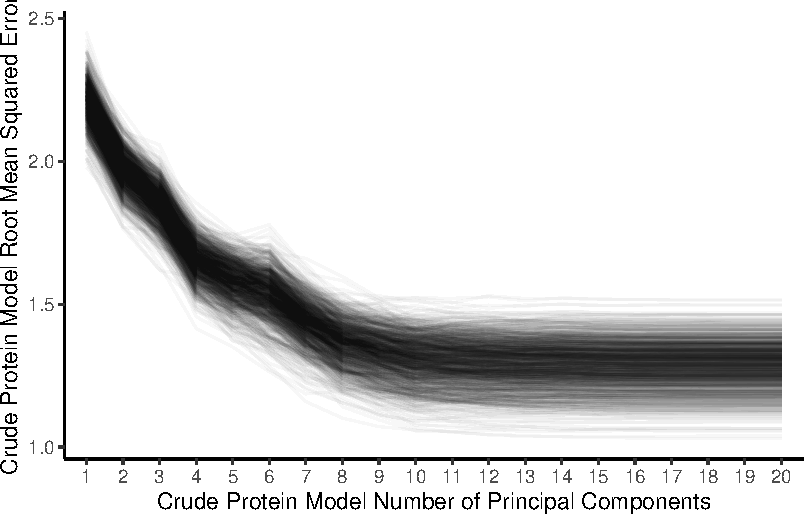
\includegraphics{index_files/figure-pdf/fig-model-calibration-1.pdf}

}

\caption{\label{fig-model-calibration}Decreasing RMSE with increasing
number of components}

\end{figure}%

\textsubscript{Source:
\href{https://rvcrawford.github.io/glowing-system/index.qmd.html}{Article
Notebook}}

\textsubscript{Source:
\href{https://rvcrawford.github.io/glowing-system/index.qmd.html}{Article
Notebook}}

\textsubscript{Source:
\href{https://rvcrawford.github.io/glowing-system/index.qmd.html}{Article
Notebook}}

The final models performances on the test sets were similar, but not
identical to, those obtained during the initial comparison of
preprocessing methods. The final models' mean RMSE was 1.03,
R\textsuperscript{2} was 0.83, RPD was 2.44, and RPIQ was 3.89. Five
percent of the models were excellent by both metrics, with RPD
\textgreater{} 3 and RPIQ \textgreater{} 4.1, while an additional 11\%
of the models were ``good'' by both metrics (RPD range from 2.5 - 3.0,
RPIQ range from 2.3 - 4.1). Forty-nine percent of the models had the
ability to approximate quantitative prediction (RPD range from 2.0 -
2.5), and 9\% of the models were able to distinguish between higher and
lower \%CP values (RPD range from 1.5 - 2.0). Therefore, 74\% of the
models had, at minimum, the ability to distinguish between high and low
values with with two thirds of them having, at minimum, the ability to
approximate quantitative prediction. Despite the generally good model
performance, a subset of poor models can be seen. For example,
Figure~\ref{fig-final-metric-boxplot} shows twenty-one models with
R\textsuperscript{2} below 0.7.

\textsubscript{Source:
\href{https://rvcrawford.github.io/glowing-system/index.qmd.html}{Article
Notebook}}

\phantomsection\label{cell-fig-final-metric-boxplot}
\begin{figure}[H]

\centering{

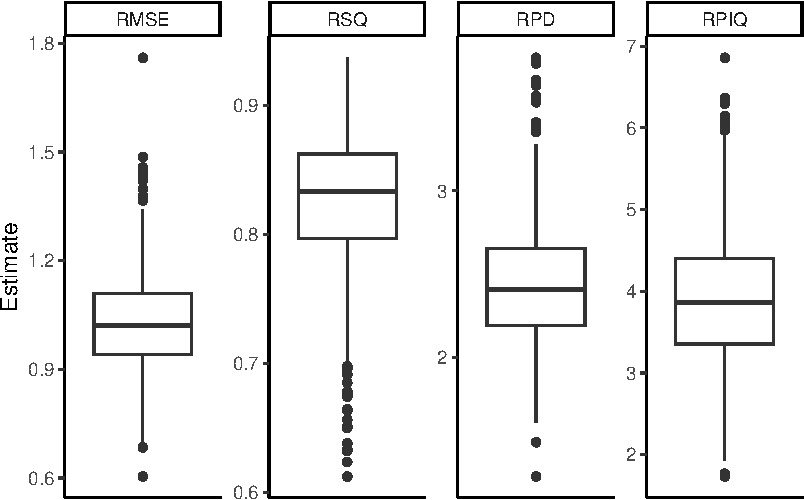
\includegraphics{index_files/figure-pdf/fig-final-metric-boxplot-1.pdf}

}

\caption{\label{fig-final-metric-boxplot}Final model test set
performance (1000 iterations)}

\end{figure}%

\textsubscript{Source:
\href{https://rvcrawford.github.io/glowing-system/index.qmd.html}{Article
Notebook}}

\textsubscript{Source:
\href{https://rvcrawford.github.io/glowing-system/index.qmd.html}{Article
Notebook}}

\textsubscript{Source:
\href{https://rvcrawford.github.io/glowing-system/index.qmd.html}{Article
Notebook}}

\textsubscript{Source:
\href{https://rvcrawford.github.io/glowing-system/index.qmd.html}{Article
Notebook}}

\textsubscript{Source:
\href{https://rvcrawford.github.io/glowing-system/index.qmd.html}{Article
Notebook}}

\textsubscript{Source:
\href{https://rvcrawford.github.io/glowing-system/index.qmd.html}{Article
Notebook}}

\textsubscript{Source:
\href{https://rvcrawford.github.io/glowing-system/index.qmd.html}{Article
Notebook}}

Finally, the pattern of test set errors was examined on a per-sample
basis by calculating the difference between the actual and predicted
values for the samples in the test sets
Figure~\ref{fig-validation_set_performance} . A linear model was fit
considering the mean estimated error for each sample where that sample
was in the test set as compared to the sample's actual value. The models
overestimated \%CP by approximately 0.5 \% in the lowest tertile and
underestimated \%CP by -0.01 \% and -0.41 \% in the middle and highest
tertile, respectively. The variance of the errors did not increase
appreciably as \%CP increased.

\phantomsection\label{cell-fig-validation_set_performance}
\begin{figure}[H]

\centering{

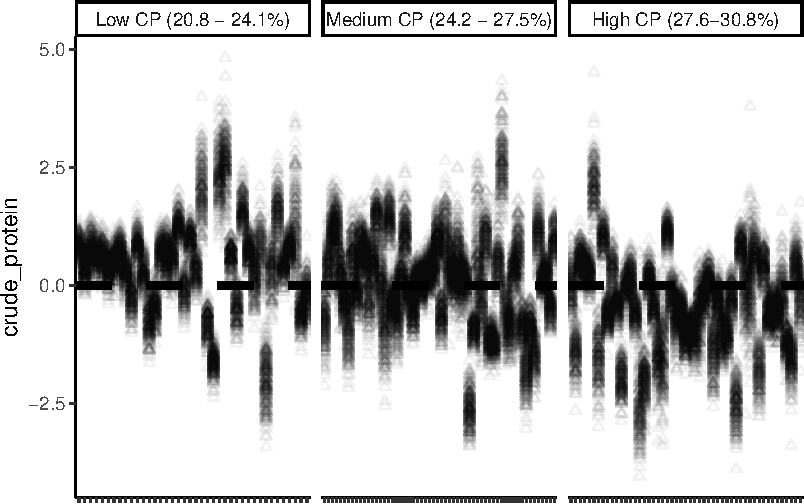
\includegraphics{index_files/figure-pdf/fig-validation_set_performance-1.pdf}

}

\caption{\label{fig-validation_set_performance}Test set prediction
errors on a per-sample basis. Actual sample value set to 0, and samples
ranked from least to greatest actual \% CP value}

\end{figure}%

\textsubscript{Source:
\href{https://rvcrawford.github.io/glowing-system/index.qmd.html}{Article
Notebook}}

\textsubscript{Source:
\href{https://rvcrawford.github.io/glowing-system/index.qmd.html}{Article
Notebook}}

The 15 (10\%) best and 15 worst predicted samples as measured by the
mean absolute error of prediction were identified and their backgrounds
examined. Overall, half of the samples in the data set came from Ithaca,
NY (``Ithaca''), while 28\% were collected from Geneva, NY (``Geneva'')
Table~\ref{tbl-hemp_provenance}. However, of the 15 worst-predicted
samples, 9 were from Geneva, while 3 of the 15 best-predicted samples
were from Geneva (by contrast, 7 of the best-predicted and 5 of the
worst-predicted samples came from Ithaca). Overall, samples from Geneva
had the highest mean absolute error of prediction among locations, 61\%
greater than samples from Ithaca and 155\% greater than samples from
Freeville, NY (the only locations with more than 20 samples).

This study is limited in that it represents the creation of one model
based upon spectra collected from one machine. NIRS calibrations can be
unique to a particular machine, even if the machines compared are of the
same model (Reeves, 2012). As well, the calibration and validation sets
are relatively small.

This research showed the promise of the use of NIRS in order to make
predictions concerning \%CP in hemp grain using PLS. Promising
preprocessing methods were identified and a model was validated. Further
research could refine a \%CP model by including more samples,
particularly by rectifying the class imbalance between Geneva and
Ithaca, identifying promising spectral regions, or by examining other
predictive methods.

\subsection{ACKNOWLEDGMENTS}\label{acknowledgments}

This work would not have been possible without the efforts of the field
staff, undergraduate, and graduate students who planted, maintained,
monitored and harvested these trials.

\subsection{CONFLICT OF INTEREST}\label{conflict-of-interest}

The authors declare no conflict of interest.

\subsection{ORCID}\label{orcid}

\subsection{SUPPLEMENTAL MATERIAL}\label{supplemental-material}

\begin{longtable}[]{@{}lrrrrrr@{}}

\caption{\label{tbl-hemp_provenance}Tally of hemp cultivars and
locations. Private cultivars are labeled ``Cultivar1'', ``Cultivar2'',
etc., while experimental cultivars are labeled ``Experimental1'',
``Experimental2'', etc.}

\tabularnewline

\toprule\noalign{}
Cultivar & Chazy & Freeville & Geneva & Ithaca & Willsboro & Total \\
\midrule\noalign{}
\endhead
\bottomrule\noalign{}
\endlastfoot
ALTAIR & & & & 1 & & 1 \\
ANKA & & 1 & 3 & 5 & 2 & 11 \\
BIALOBRZESKIE & & 1 & 3 & 4 & 1 & 9 \\
CANDA & & 1 & 1 & 1 & & 3 \\
CFX-1 & & 1 & 2 & 5 & & 8 \\
CFX-2 & & 1 & 2 & 4 & & 7 \\
CRS-1 & 1 & 1 & 2 & 5 & & 9 \\
CULTIVAR1 & & 1 & & & & 1 \\
CULTIVAR2 & & & & 1 & & 1 \\
CULTIVAR3 & & & & 1 & & 1 \\
CULTIVAR4 & & & & 1 & & 1 \\
EARLINA 8 & & & 1 & & & 1 \\
EXPERIMENTAL1 & & & & 1 & & 1 \\
EXPERIMENTAL2 & & & & 1 & & 1 \\
FELINA 32 & & 1 & 2 & 3 & & 6 \\
FUTURA 75 & & 1 & 3 & 4 & & 8 \\
GRANDI & & 3 & 3 & 4 & & 10 \\
H-51 & & & 1 & 2 & & 3 \\
HAN-FN-H & & & & 1 & & 1 \\
HAN-NW & & & & 1 & & 1 \\
HELENA & & 1 & & & & 1 \\
HENOLA & & & & 2 & & 2 \\
HLESIA & & & & 3 & & 3 \\
HLIANA & & & 1 & 1 & & 2 \\
JOEY & & 1 & 1 & 1 & & 3 \\
KATANI & & 2 & 3 & 4 & & 9 \\
NEBRASKA (FERAL) & 1 & & & 1 & & 2 \\
PEWTER RIVER & & 1 & & & & 1 \\
PICOLO & & 1 & 2 & 5 & & 8 \\
PORTUGAL & & & 1 & & & 1 \\
ROCKY HEMP & & & 1 & & & 1 \\
STERLING GOLD & & & 1 & & & 1 \\
SWIFT & 1 & 1 & & 1 & & 3 \\
TYGRA & & 1 & 3 & 4 & & 8 \\
USO-31 & 2 & 1 & 2 & 4 & & 9 \\
WOJKO & & 1 & 3 & 4 & & 8 \\
X-59 & & 2 & & 1 & & 3 \\
TOTAL & 5 & 24 & 41 & 76 & 3 & 149 \\

\end{longtable}

\textsubscript{Source:
\href{https://rvcrawford.github.io/glowing-system/index.qmd.html}{Article
Notebook}}

\subsection{OPTIONAL SECTIONS}\label{optional-sections}

\subsection{REFERENCES}\label{references}

\subsection*{FIGURES AND TABLES}\label{figures-and-tables}
\addcontentsline{toc}{subsection}{FIGURES AND TABLES}

\phantomsection\label{refs}
\begin{CSLReferences}{1}{0}
\bibitem[\citeproctext]{ref-barnes_standard_1989}
Barnes, R. J., Dhanoa, M. S., \& Lister, S. J. (1989). Standard {Normal}
{Variate} {Transformation} and {De}-{Trending} of {Near}-{Infrared}
{Diffuse} {Reflectance} {Spectra}. \emph{Applied Spectroscopy},
\emph{43}(5), 772--777. \url{https://doi.org/10.1366/0003702894202201}

\bibitem[\citeproctext]{ref-datatable}
Barrett, T., Dowle, M., Srinivasan, A., Gorecki, J., Chirico, M., \&
Hocking, T. (2024). \emph{{data.table}: Extension of
{``{data.frame}''}}. \url{https://CRAN.R-project.org/package=data.table}

\bibitem[\citeproctext]{ref-barta_proteomic_2024}
Bárta, J., Roudnický, P., Jarošová, M., Zdráhal, Z., Stupková, A.,
Bártová, V., Krejčová, Z., Kyselka, J., Filip, V., Říha, V., Lorenc, F.,
Bedrníček, J., \& Smetana, P. (2024). Proteomic {Profiles} of {Whole}
{Seeds}, {Hulls}, and {Dehulled} {Seeds} of {Two} {Industrial} {Hemp}
({Cannabis} sativa {L}.) {Cultivars}. \emph{Plants}, \emph{13}(1), 111.
\url{https://doi.org/10.3390/plants13010111}

\bibitem[\citeproctext]{ref-bellon-maurel_critical_2010}
Bellon-Maurel, V., Fernandez-Ahumada, E., Palagos, B., Roger, J.-M., \&
McBratney, A. (2010). Critical review of chemometric indicators commonly
used for assessing the quality of the prediction of soil attributes by
{NIR} spectroscopy. \emph{TrAC Trends in Analytical Chemistry},
\emph{29}(9), 1073--1081.
\url{https://doi.org/10.1016/j.trac.2010.05.006}

\bibitem[\citeproctext]{ref-callaway_hempseed_2004}
Callaway, J. C. (2004). Hempseed as a nutritional resource: {An}
overview. \emph{Euphytica}, \emph{140}(1), 65--72.
\url{https://doi.org/10.1007/s10681-004-4811-6}

\bibitem[\citeproctext]{ref-chadalavada_nir_2022}
Chadalavada, K., Anbazhagan, K., Ndour, A., Choudhary, S., Palmer, W.,
Flynn, J. R., Mallayee, S., Pothu, S., Prasad, K. V. S. V.,
Varijakshapanikar, P., Jones, C. S., \& Kholová, J. (2022). {NIR}
{Instruments} and {Prediction} {Methods} for {Rapid} {Access} to {Grain}
{Protein} {Content} in {Multiple} {Cereals}. \emph{Sensors (Basel,
Switzerland)}, \emph{22}(10). \url{https://doi.org/10.3390/s22103710}

\bibitem[\citeproctext]{ref-ely_industrial_2022}
Ely, K., \& Fike, J. (2022). Industrial {Hemp} and {Hemp} {Byproducts}
as {Sustainable} {Feedstuffs} in {Livestock} {Diets}. In D. C. Agrawal,
R. Kumar, \& M. Dhanasekaran (Eds.), \emph{Cannabis/{Hemp} for
{Sustainable} {Agriculture} and {Materials}} (pp. 145--162). Springer.
\url{https://doi.org/10.1007/978-981-16-8778-5_6}

\bibitem[\citeproctext]{ref-garrido-varo_note_2019}
Garrido-Varo, A., Garcia-Olmo, J., \& Fearn, T. (2019). A note on
{Mahalanobis} and related distance measures in {WinISI} and {The}
{Unscrambler}. \emph{Journal of Near Infrared Spectroscopy},
\emph{27}(4), 253--258. \url{https://doi.org/10.1177/0967033519848296}

\bibitem[\citeproctext]{ref-geyer_genetics_2022}
Geyer, M., Mohler, V., \& Hartl, L. (2022). Genetics of the {Inverse}
{Relationship} between {Grain} {Yield} and {Grain} {Protein} {Content}
in {Common} {Wheat}. \emph{Plants}, \emph{11}(16), 2146.
\url{https://doi.org/10.3390/plants11162146}

\bibitem[\citeproctext]{ref-giancaspro_genetic_2019}
Giancaspro, A., Giove, S. L., Blanco, A., \& Gadaleta, A. (2019).
Genetic {Variation} for {Protein} {Content} and {Yield}-{Related}
{Traits} in a {Durum} {Population} {Derived} {From} an
{Inter}-{Specific} {Cross} {Between} {Hexaploid} and {Tetraploid}
{Wheat} {Cultivars}. \emph{Frontiers in Plant Science}, \emph{10}.
\url{https://doi.org/10.3389/fpls.2019.01509}

\bibitem[\citeproctext]{ref-hayes_measuring_2020}
Hayes, M. (2020). Measuring {Protein} {Content} in {Food}: {An}
{Overview} of {Methods}. \emph{Foods}, \emph{9}(10), 1340.
\url{https://doi.org/10.3390/foods9101340}

\bibitem[\citeproctext]{ref-tidymodels}
Kuhn, M., \& Wickham, H. (2020). \emph{{Tidymodels}: A collection of
packages for modeling and machine learning using tidyverse principles.}
\url{https://www.tidymodels.org}

\bibitem[\citeproctext]{ref-caret}
Kuhn, \& Max. (2008). Building predictive models in r using the caret
package. \emph{Journal of Statistical Software}, \emph{28}(5), 1--26.
\url{https://doi.org/10.18637/jss.v028.i05}

\bibitem[\citeproctext]{ref-emmeans}
Lenth, R. V. (2024). \emph{{emmeans}: Estimated marginal means, aka
least-squares means}. \url{https://CRAN.R-project.org/package=emmeans}

\bibitem[\citeproctext]{ref-li_quantitative_2020}
Li, Y., Huang, Y., Xia, J., Xiong, Y., \& Min, S. (2020). Quantitative
analysis of honey adulteration by spectrum analysis combined with
several high-level data fusion strategies. \emph{Vibrational
Spectroscopy}, \emph{108}, 103060.
\url{https://doi.org/10.1016/j.vibspec.2020.103060}

\bibitem[\citeproctext]{ref-pls}
Liland, K. H., Mevik, B.-H., \& Wehrens, R. (2023). \emph{{pls}: Partial
least squares and principal component regression}.
\url{https://CRAN.R-project.org/package=pls}

\bibitem[\citeproctext]{ref-luce_prediction_2017}
Luce, M. S., Ziadi, N., Gagnon, B., \& Lévesque, V. (2017). Prediction
of total carbon, total nitrogen, and {pH} of organic materials using
visible near-infrared reflectance spectroscopy. \emph{Canadian Journal
of Soil Science}, \emph{98}(1), 175--179.
\url{https://doi.org/10.1139/cjss-2017-0109}

\bibitem[\citeproctext]{ref-luo_properties_2005}
Luo, J., Ying, K., He, P., \& Bai, J. (2005). Properties of
{Savitzky}--{Golay} digital differentiators. \emph{Digital Signal
Processing}, \emph{15}(2), 122--136.
\url{https://doi.org/10.1016/j.dsp.2004.09.008}

\bibitem[\citeproctext]{ref-nlme2000}
Pinheiro, J. C., \& Bates, D. M. (2000). \emph{Mixed-effects models in s
and s-PLUS}. Springer. \url{https://doi.org/10.1007/b98882}

\bibitem[\citeproctext]{ref-nlme2023}
Pinheiro, J., Bates, D., \& R Core Team. (2023). \emph{{nlme}: Linear
and nonlinear mixed effects models}.
\url{https://CRAN.R-project.org/package=nlme}

\bibitem[\citeproctext]{ref-base}
R Core Team. (2024). \emph{{R}: A language and environment for
statistical computing}. R Foundation for Statistical Computing.
\url{https://www.R-project.org/}

\bibitem[\citeproctext]{ref-rawal_visible_2024}
Rawal, A., Hartemink, A., Zhang, Y., Wang, Y., Lankau, R. A., \& Ruark,
M. D. (2024). Visible and near-infrared spectroscopy predicted leaf
nitrogen contents of potato varieties under different growth and
management conditions. \emph{Precision Agriculture}, \emph{25}(2),
751--770. \url{https://doi.org/10.1007/s11119-023-10091-z}

\bibitem[\citeproctext]{ref-reeves_potential_2012}
Reeves, J. B. (2012). Potential of {Near}- and {Mid}-infrared
{Spectroscopy} in {Biofuel} {Production}. \emph{Communications in Soil
Science and Plant Analysis}, \emph{43}(1-2), 478--495.
\url{https://doi.org/10.1080/00103624.2012.641844}

\bibitem[\citeproctext]{ref-rinnan_review_2009}
Rinnan, Å., Berg, F. van den, \& Engelsen, S. B. (2009). Review of the
most common pre-processing techniques for near-infrared spectra.
\emph{TrAC Trends in Analytical Chemistry}, \emph{28}(10), 1201--1222.
\url{https://doi.org/10.1016/j.trac.2009.07.007}

\bibitem[\citeproctext]{ref-roberts_near-infrared_2004}
Roberts, C. A., Workman, J., \& Reeves, J. B. (2004).
\emph{Near-infrared spectroscopy in agriculture}. American Society of
Agronomy.

\bibitem[\citeproctext]{ref-prospectr}
Stevens, A., \& Ramirez-Lopez, L. (2024). \emph{An introduction to the
prospectr package}.

\bibitem[\citeproctext]{ref-skimr}
Waring, E., Quinn, M., McNamara, A., Arino de la Rubia, E., Zhu, H., \&
Ellis, S. (2022). \emph{{skimr}: Compact and flexible summaries of
data}. \url{https://CRAN.R-project.org/package=skimr}

\bibitem[\citeproctext]{ref-tidyverse}
Wickham, H., Averick, M., Bryan, J., Chang, W., McGowan, L. D.,
François, R., Grolemund, G., Hayes, A., Henry, L., Hester, J., Kuhn, M.,
Pedersen, T. L., Miller, E., Bache, S. M., Müller, K., Ooms, J.,
Robinson, D., Seidel, D. P., Spinu, V., \ldots{} Yutani, H. (2019).
Welcome to the {tidyverse}. \emph{Journal of Open Source Software},
\emph{4}(43), 1686. \url{https://doi.org/10.21105/joss.01686}

\bibitem[\citeproctext]{ref-williams_application_1975}
Williams, P. C. (1975). Application of near infrared reflectance
spectroscopy to analysis of cereal grains and oilseeds. \emph{Cereal
Chemistry}, \emph{52}(4 p.561-576), 576--561.

\bibitem[\citeproctext]{ref-wold_pls-regression_2001}
Wold, S., Sjöström, M., \& Eriksson, L. (2001). {PLS}-regression: A
basic tool of chemometrics. \emph{Chemometrics and Intelligent
Laboratory Systems}, \emph{58}(2), 109--130.
\url{https://doi.org/10.1016/S0169-7439(01)00155-1}

\end{CSLReferences}



\end{document}
